\documentclass[a4paper]{scrartcl}
\usepackage[a4paper,margin=0cm,left=-0.65cm]{geometry}
\usepackage{amssymb,amsmath}

\usepackage[rgb]{xcolor}
\usepackage{tikz}
\usetikzlibrary{shadings}

\begin{document}
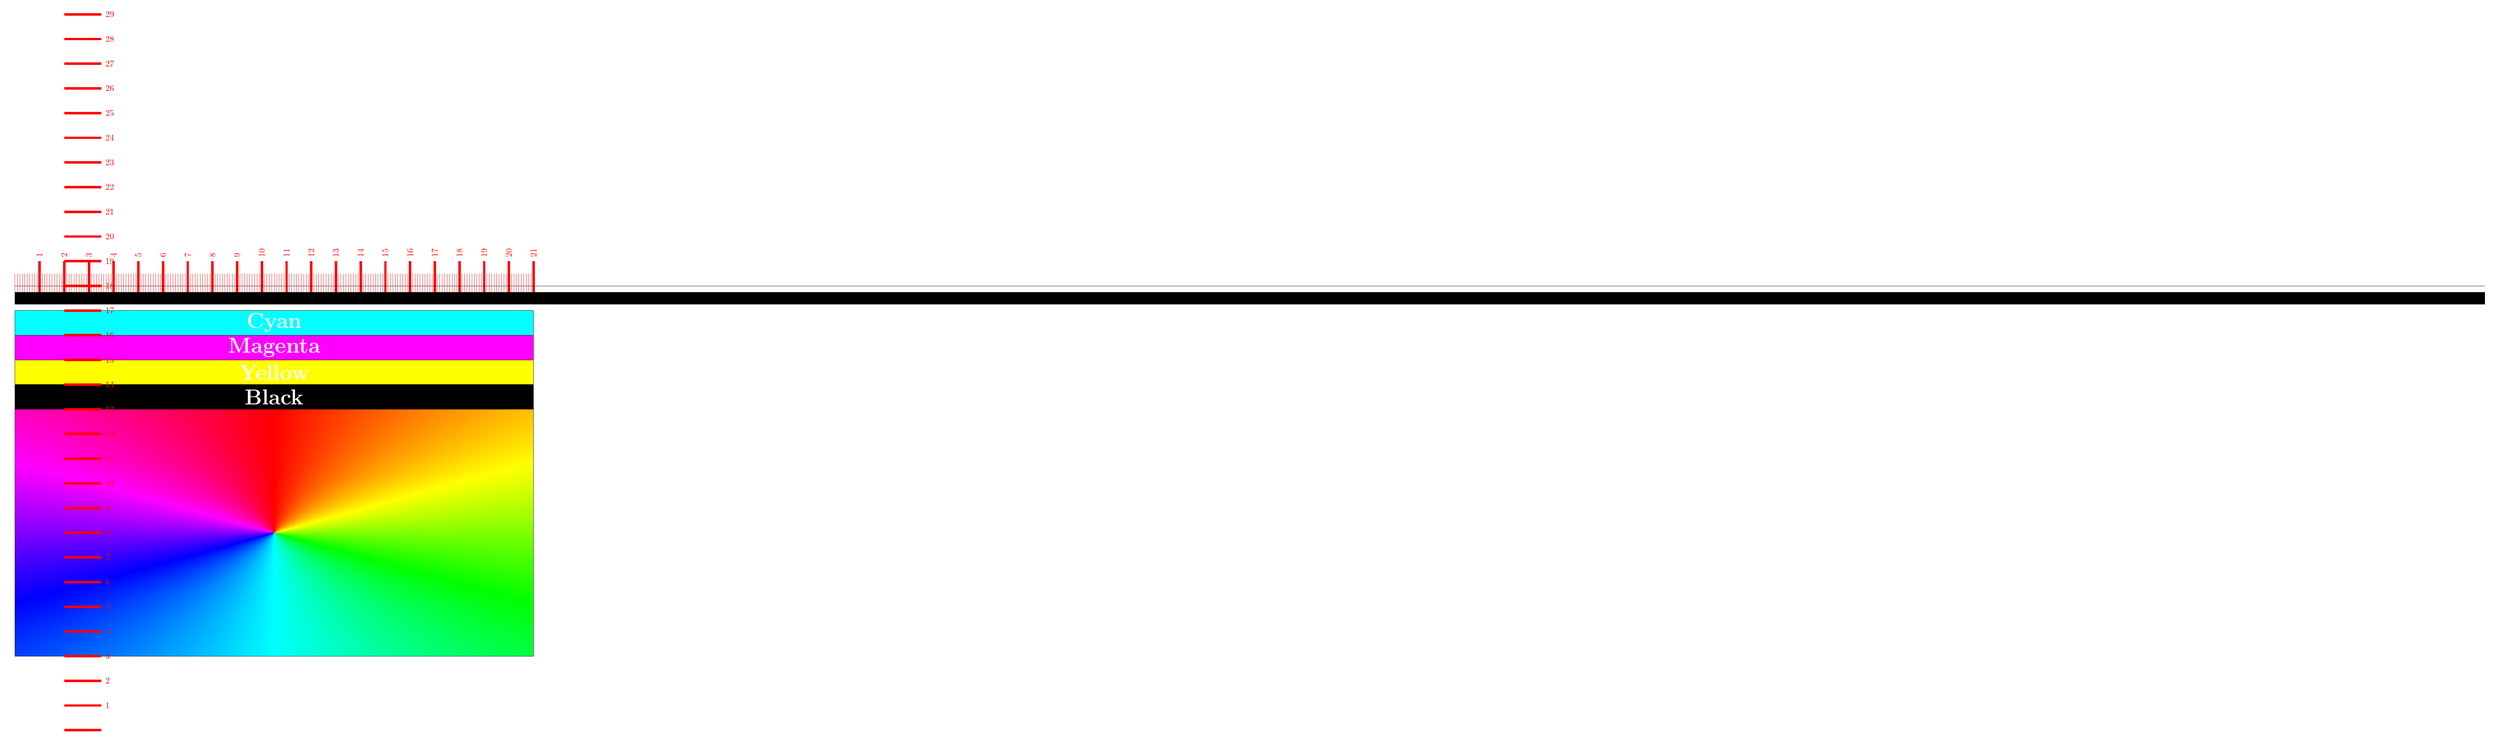
\begin{tikzpicture}
    \begin{scope}[yshift=3cm]
        \draw[shading=color wheel] (0,0) rectangle (20.998,10);
    \end{scope}
    \begin{scope}[yshift=3cm]
        \draw[rectangle,fill=cyan] (0,13) rectangle (20.998,14) node[pos=.5,text=white] {\Huge \textbf{Cyan}};
        \draw[rectangle,fill=magenta] (0,12) rectangle (20.998,13) node[pos=.5,text=white] {\Huge \textbf{Magenta}};
        \draw[rectangle,fill=yellow] (0,11) rectangle (20.998,12) node[pos=.5,text=white] {\Huge \textbf{Yellow}};
        \draw[rectangle,fill=black] (0,10) rectangle (20.998,11) node[pos=.5,text=white] {\Huge \textbf{Black}};
    \end{scope}
    \begin{scope}[yshift=17.5cm]
      \foreach \x in {1,2,...,21}
      \draw [color=red, line width=1mm](\x cm,0cm) -- (\x cm,1.5cm)
      node[color=red, rotate=90, anchor=west] {\pgfmathprint{int(\x)}};

      \foreach \x in {0,1,...,210}
      \draw [color=red, line width=0.1mm](\x mm,0cm) -- (\x mm,1.0cm)
      node[color=red, rotate=90, anchor=west] {};

      \draw[line width=5mm](0cm, 0cm) -- (100,0cm);
      \draw[line width=0.1mm](0cm, 0.5cm) -- (100,0.5cm);
    \end{scope}

    \draw [color=red, line width=1mm](2cm,0 cm) -- (3.5cm,0 cm)
      node[color=red, anchor=west] {};
    \foreach \y in {1,2,...,29}
      \draw [color=red, line width=1mm](2cm,\y cm) -- (3.5cm,\y cm)
      node[color=red, anchor=west] {\pgfmathprint{int(\y)}};
\end{tikzpicture}
\end{document}
